\section{Abstract}

The nucleotide frequencies in protein-coding sequences is the result of the equilibrium between mutation and selection.
As a consequence, protein-coding sequences subjected to mutational bias at the nucleotide level, and evolving under selection at the amino-acids, will lean toward lower mutational bias when observed at the protein level.
Unfortunately, parametric \gls{codon} models developed to estimate the rate of evolution on amino-acids use the observed mutational bias at the protein level and don't take into account this effect.
Thus, such parametric \gls{codon} models are inherently misspecified to untangle mutation and selection, and they don’t estimate the mutational process reliably.
We also show that even if the mutational process is misspecified, parametric \gls{codon} models are able to estimate reliably the rate of evolution acting on amino-acids.
But if one wants to also estimate the mutational process, one need to use model where the rate of evolution is a tensor (95 parameters) instead of a single parameter.


\section{Introduction}

$\bullet$ Nucleotide composition in protein-coding sequences is the result of the equilibrium between mutation and selection.

$\bullet$ Phenomenological parametric \gls{codon} models developed to estimate the rate of evolution on amino-acids are qualitative, in the sens that they model the fitness landscape and drift throught an unique aggregate parameter.

$\bullet$ By aggregating selection and drift into a sole parameter, is the mutational process estimated reliably?

$\bullet$ This model predicts that the nucleotide composition is the same for all $3$ positions of the codons, however it as empirically been observed that the nucleotide composition are not identical.

$\bullet$ Can we estimate mutational bias reliably?

$\bullet$ Is mutational bias having side effect on estimation of selection?

$\bullet$ Influence of mutation bias and hydrophobicity on the substitution rates and sequence entropies of protein evolution \citet{Santos2018}

\section{Results}

$\bullet$ Parameter of mutation, selection and drift.
One parameter for mutational bias ($\lambda$), one for selection/drift ($\alpha$) (see figure \ref{fig-mut-bias:parameters}).

$\bullet$ The mutationnal bias $\lambda = (\mutequi_A+\mutequi_T)/(\mutequi_C+\mutequi_G)$ is shared by all sites of the sequence (see section \ref{sec-mut-bias:mut-matrix}).

$\bullet$ Each site of the sequence is defined by its own fitness of amino-acid, drawn from a Dirichlet distribution of concentration parameter $\alpha$ (see section \ref{sec-mut-bias:aa-selection}).

\begin{figure}[H]
    \centering
    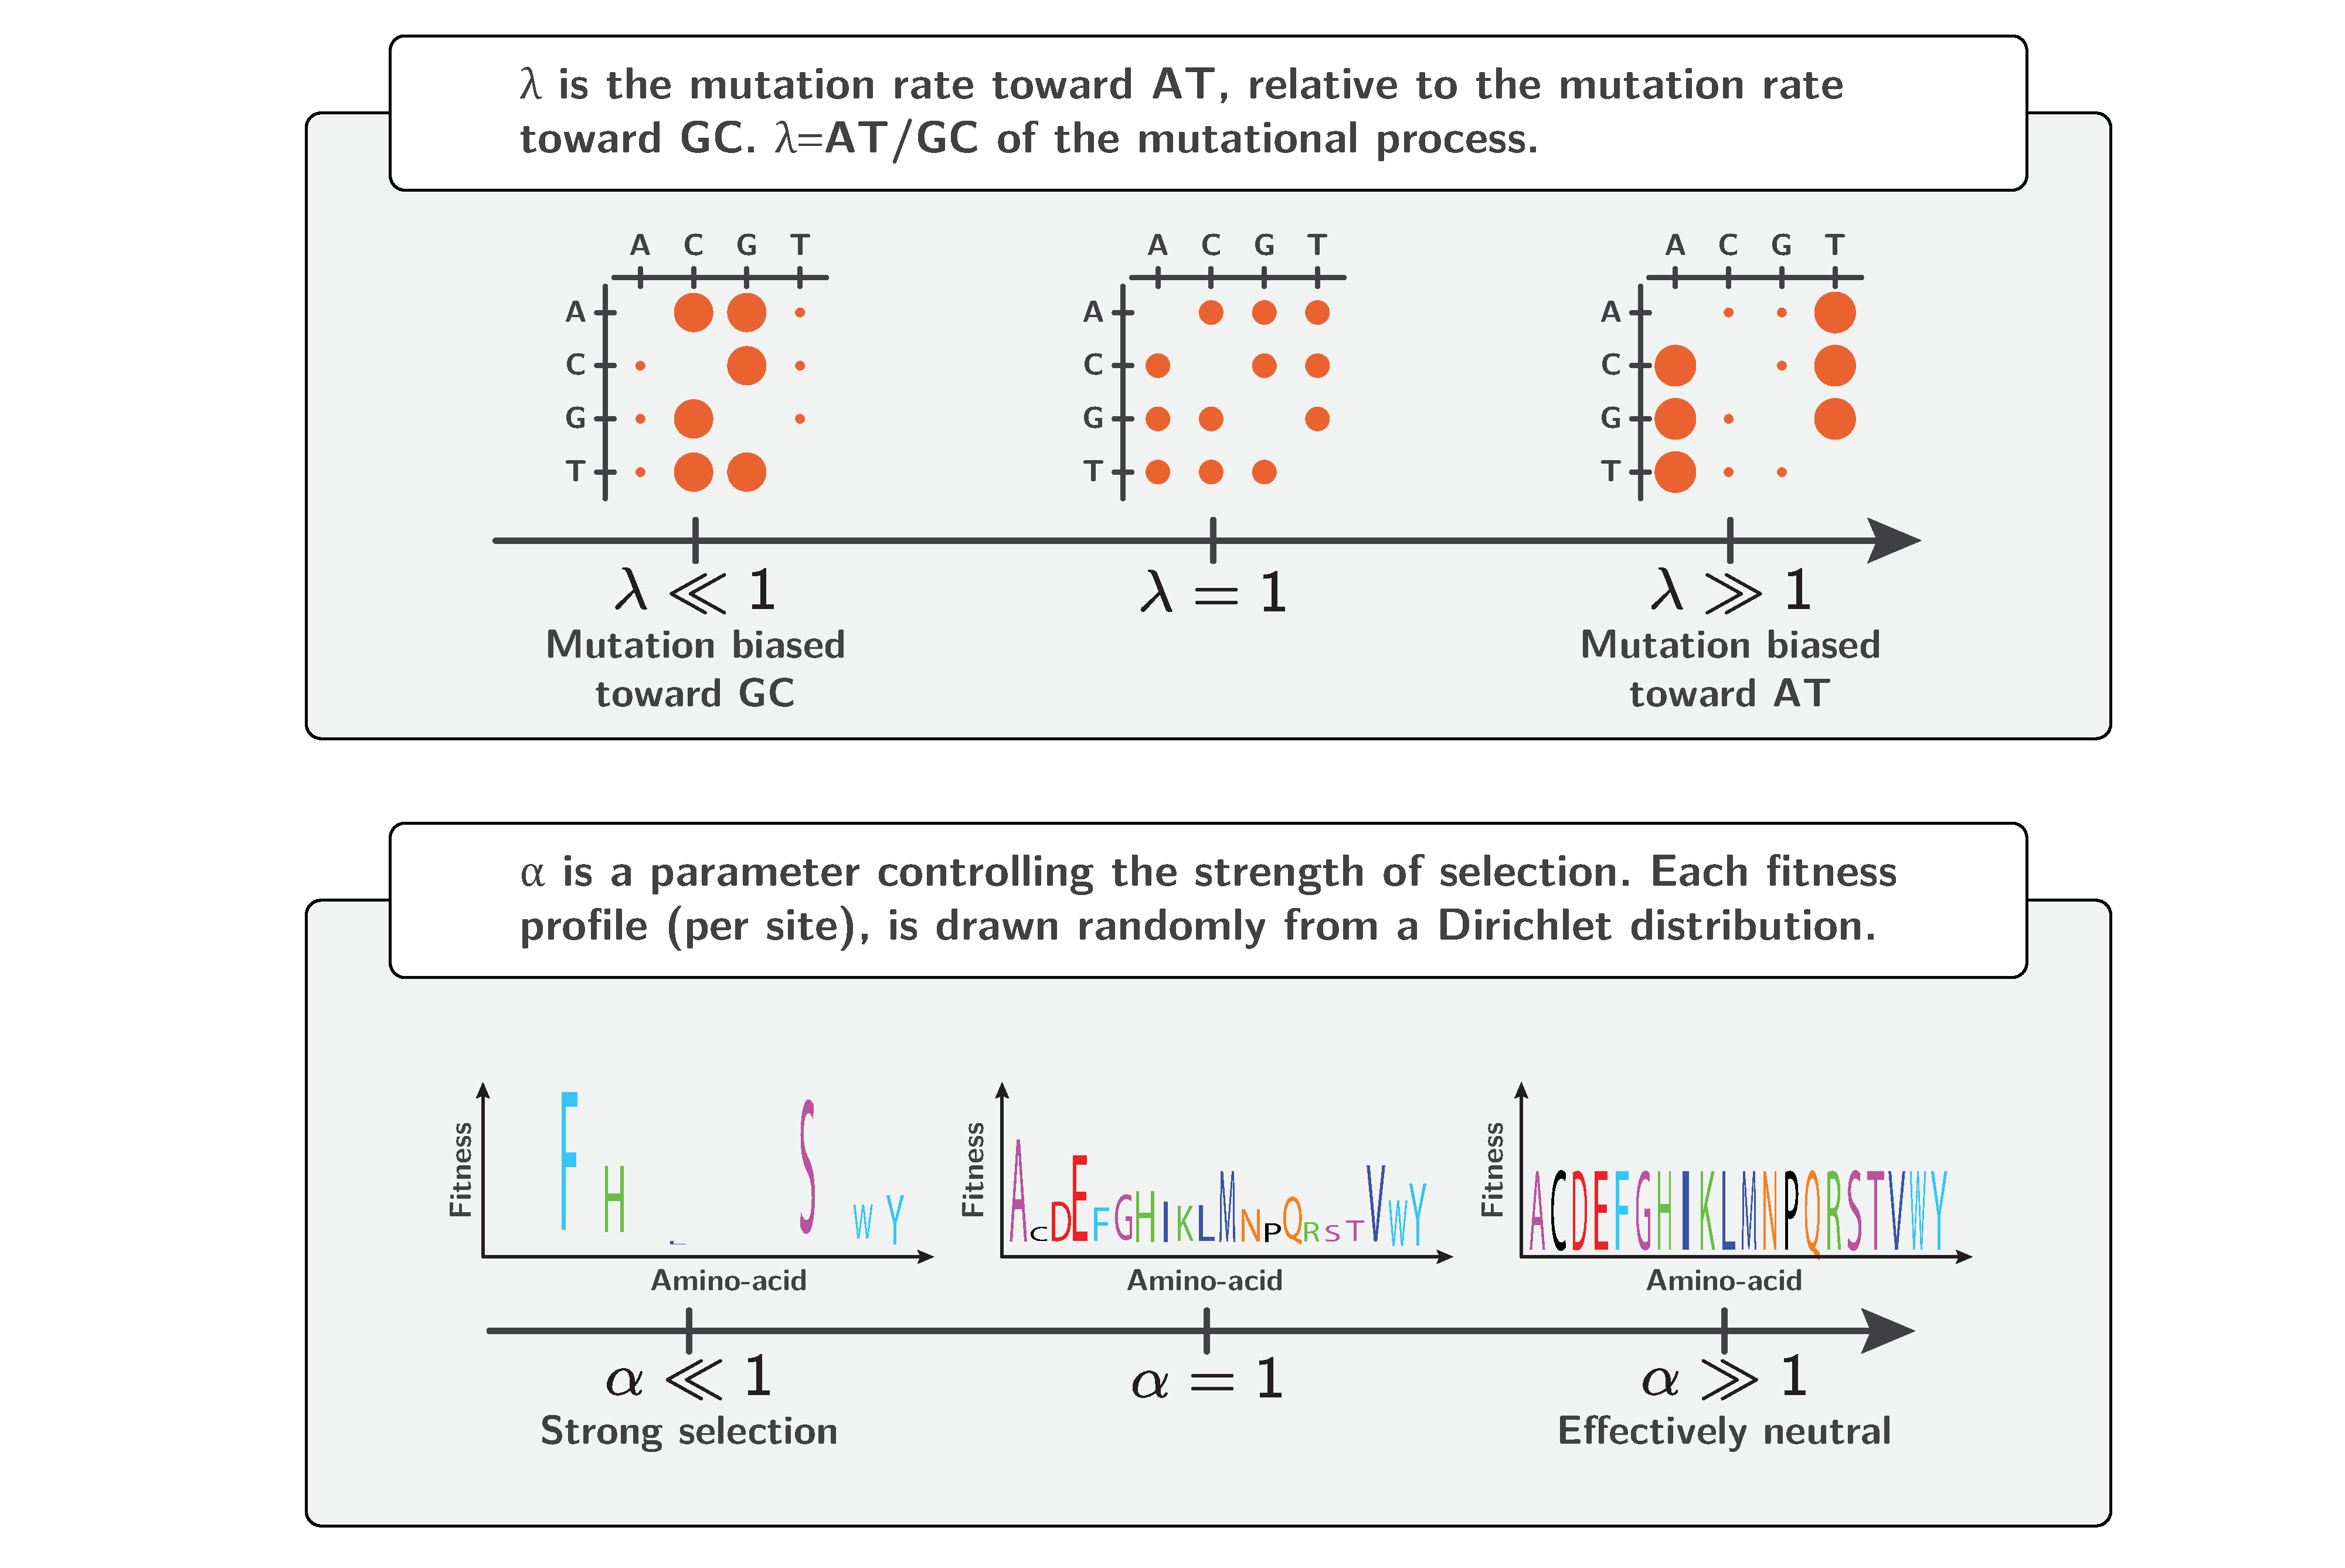
\includegraphics[width=\textwidth] {parameters}
    \caption[Parameters of the mutation-selection model]{
    Parameters of the mutation-selection model.
    One parameter for mutational bias, and one for strength of selection.}
    \label{fig-mut-bias:parameters}
\end{figure}

$\bullet$ Simulation along a species tree of the model result in a observed final alignment (see section \ref{sec-mut-bias:simu}), from which summary statistics can be computed (see figure \ref{fig-mut-bias:simulations-alignment}).

\begin{figure}[H]
    \centering
    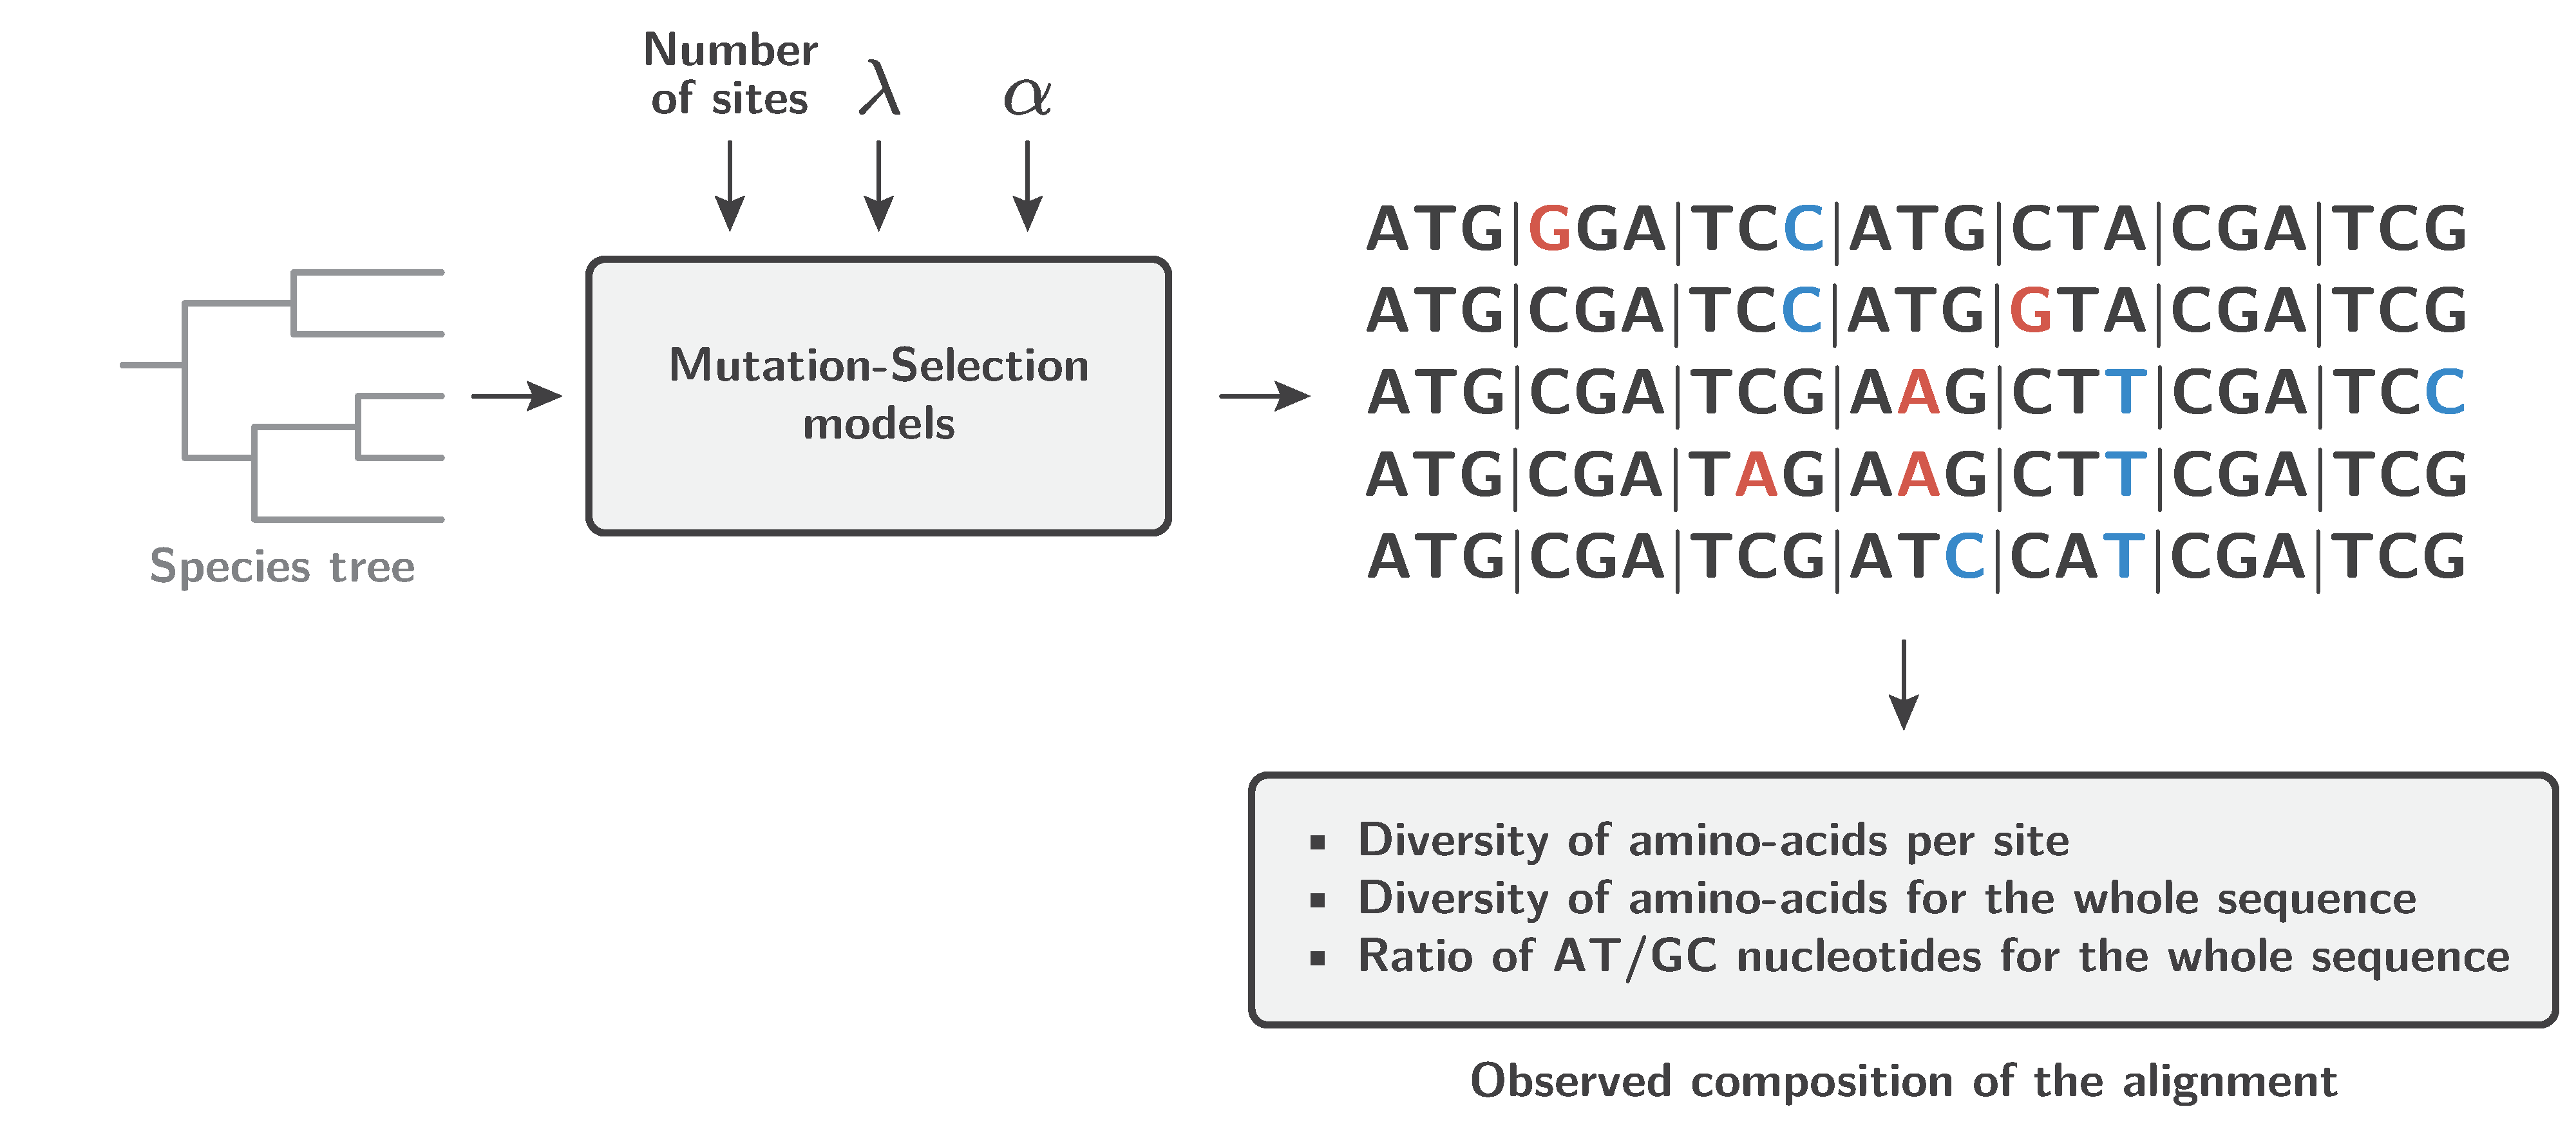
\includegraphics[width=\textwidth] {simulations-alignment}
    \caption[Simulations and analysis]{We can observe composition of the alignment as function of the mutation and selection parameters.}
    \label{fig-mut-bias:simulations-alignment}
\end{figure}

\subsection{Observed summary statistics}

$\bullet$ From the alignment, one can simply observe the frequency of the different nucleotides, and the resulting mutational bias AT/GC.

$\bullet$ Composition of the observed bias can be compared to underlying mutational bias $(\mutequi_A+\mutequi_T)/(\mutequi_C+\mutequi_G) = \lambda$ (see figure \ref{fig-mut-bias:AT-GC-obs}).
The third position matches the mutational bias, however the first and second position are impacted by the strength of selection.

\begin{figure}[H]
    \centering
    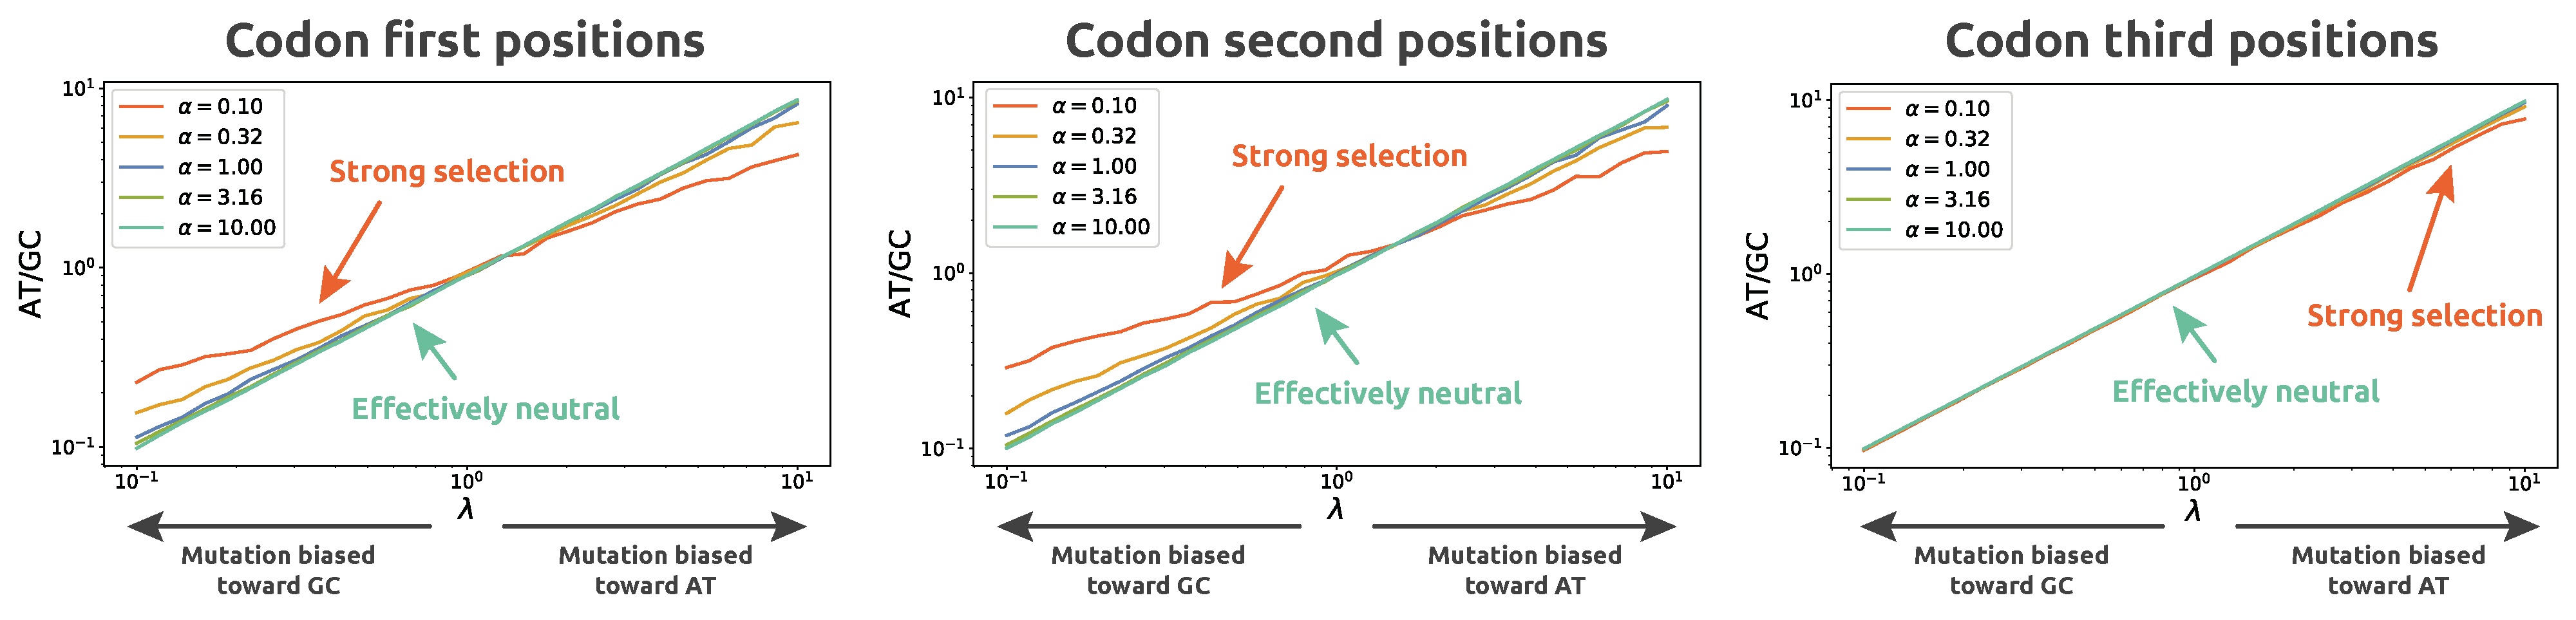
\includegraphics[width=\textwidth] {AT-GC-obs}
    \caption[AT/GC composition of the alignment]{
    AT/GC composition of the alignment.
    Observed AT/GC at the third \gls{codon} position matches the mutational bias.
    Selection is balancing the mutational bias.}
    \label{fig-mut-bias:AT-GC-obs}
\end{figure}


$\bullet$ The evolutionary variability of an amino acid site in a protein family is an important indicator of the selective constraints that the site experiences.

$\bullet$ This variability is usually quantified through the sequence entropy \citep{Goldstein2017}, either for a single site and averaged over the sequence, or directly for the all alignment.

$\bullet$ Our analysis highlights how important it is to distinguish between amino acid frequencies averaged over a large class of sites and amino acid frequencies at individual sites (see figure \ref{fig-mut-bias:diversity-aa}).

$\bullet$ For example, all amino acids occur at comparable frequencies in the alignment, yet at any given site, only a small number of amino acids are actually permissible \citep{Ramsey2011}.

$\bullet$ The mutationnal bias greatly reduce site and sequence entropy.

\begin{figure}[H]
    \centering
    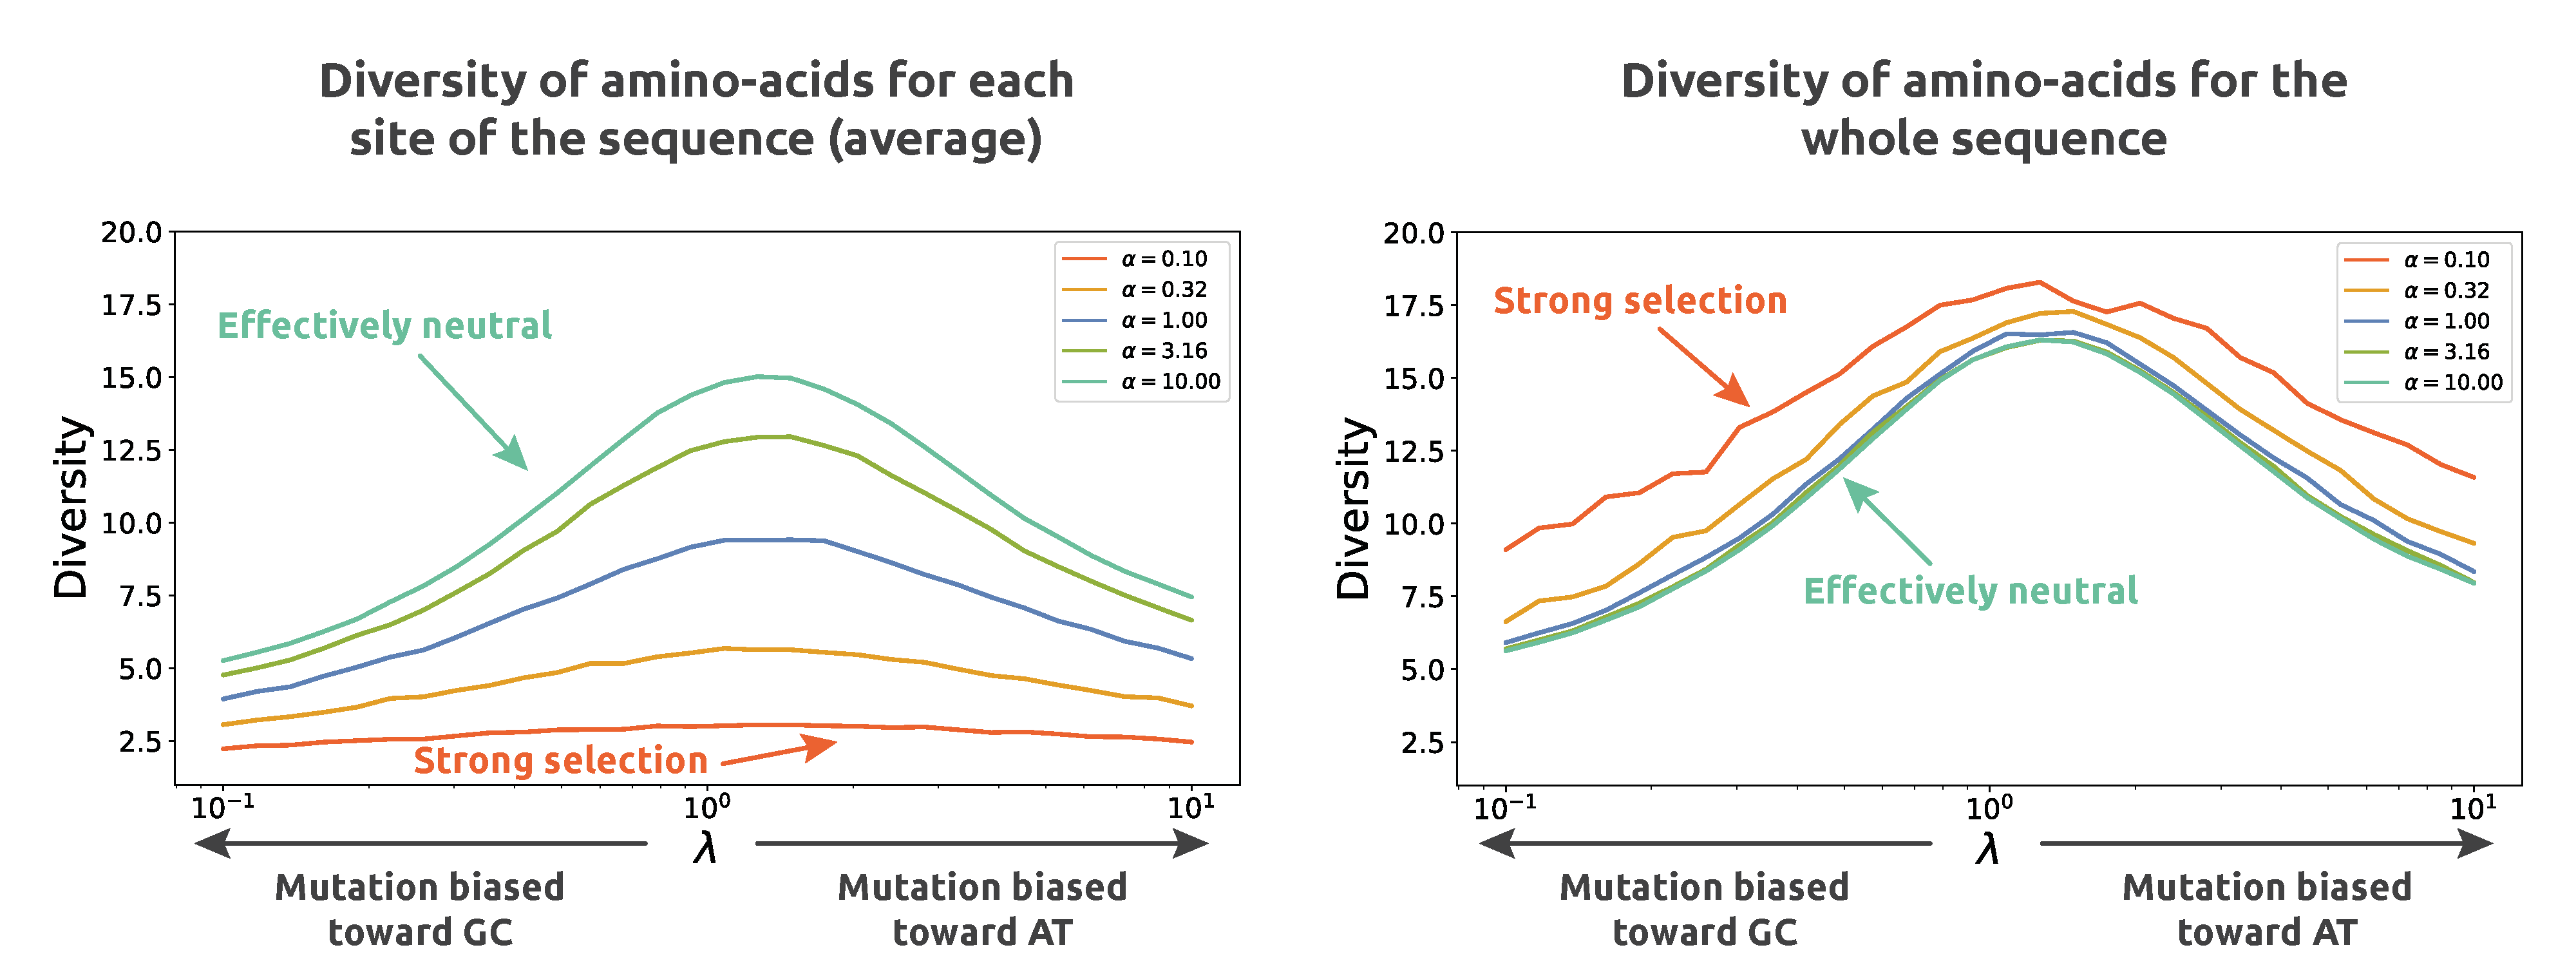
\includegraphics[width=\textwidth] {diversity-aa}
    \caption[Diversity of amino-acids]{
    Diversity of amino-acids, computed as the entropy of the amino-acid frequencies.
    Sequence-diversity is higher than site-diversity, because at any given site only a small number of amino acids are actually permissible.
    Diversity decreases with mutational bias.
    Site-diversity decreases with selection.
    Sequence-diversity increase with selection.}
    \label{fig-mut-bias:diversity-aa}
\end{figure}

%Evolutionary rate, which measures the rate at which mutations at individual sites arise and go to fixation, is governed by the amino acid distribution of individual sites, not the average distribution over a broad class of sites.
%The \gls{substitution} rate (e.g., Grishin, Wolf \& Koonin, 2000).
%These two measures of evolutionary variability are considered to be essentially equivalent \citep{Halpern1998}, though they are differently influenced by the mutational process \citep{Santos2018}.

$\bullet$ Because the sequences are not independent but related together by a specie tree, entropy of the alignment does not converges to entropy of the substitution process.

$\bullet$ Instead, the substitution rate $\omega$, which measures the rate at which mutations at individual sites arise and go to fixation, is an aggregate parameter measuring the overall strength of selection of the sequence.

$\bullet$ Because point substitutions are recorded along the simulation, the average substitution rate can be quantified (see figure \ref{fig-mut-bias:definitions-omega}).

\begin{figure}[H]
    \centering
    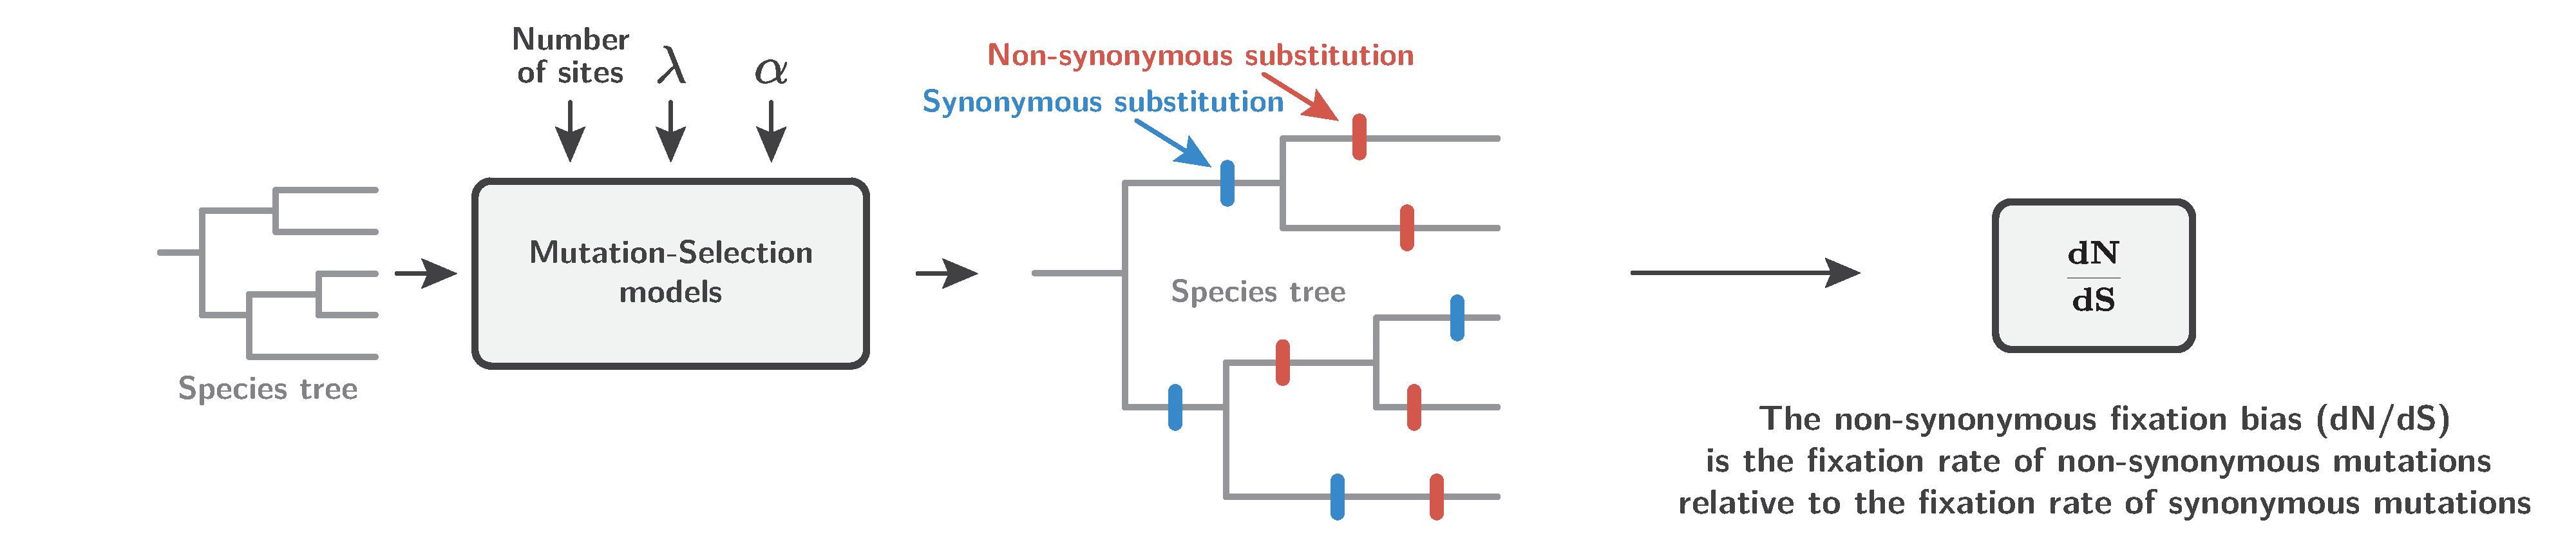
\includegraphics[width=\textwidth] {definitions-omega}
    \caption[Definition of $\omega$]{Definition of $\omega$.}
    \label{fig-mut-bias:definitions-omega}
\end{figure}

$\bullet$ Substitution rate depends strongly on selection/drift, but not on mutational bias (see figure \ref{fig-mut-bias:omega}).

\begin{figure}[H]
    \centering
    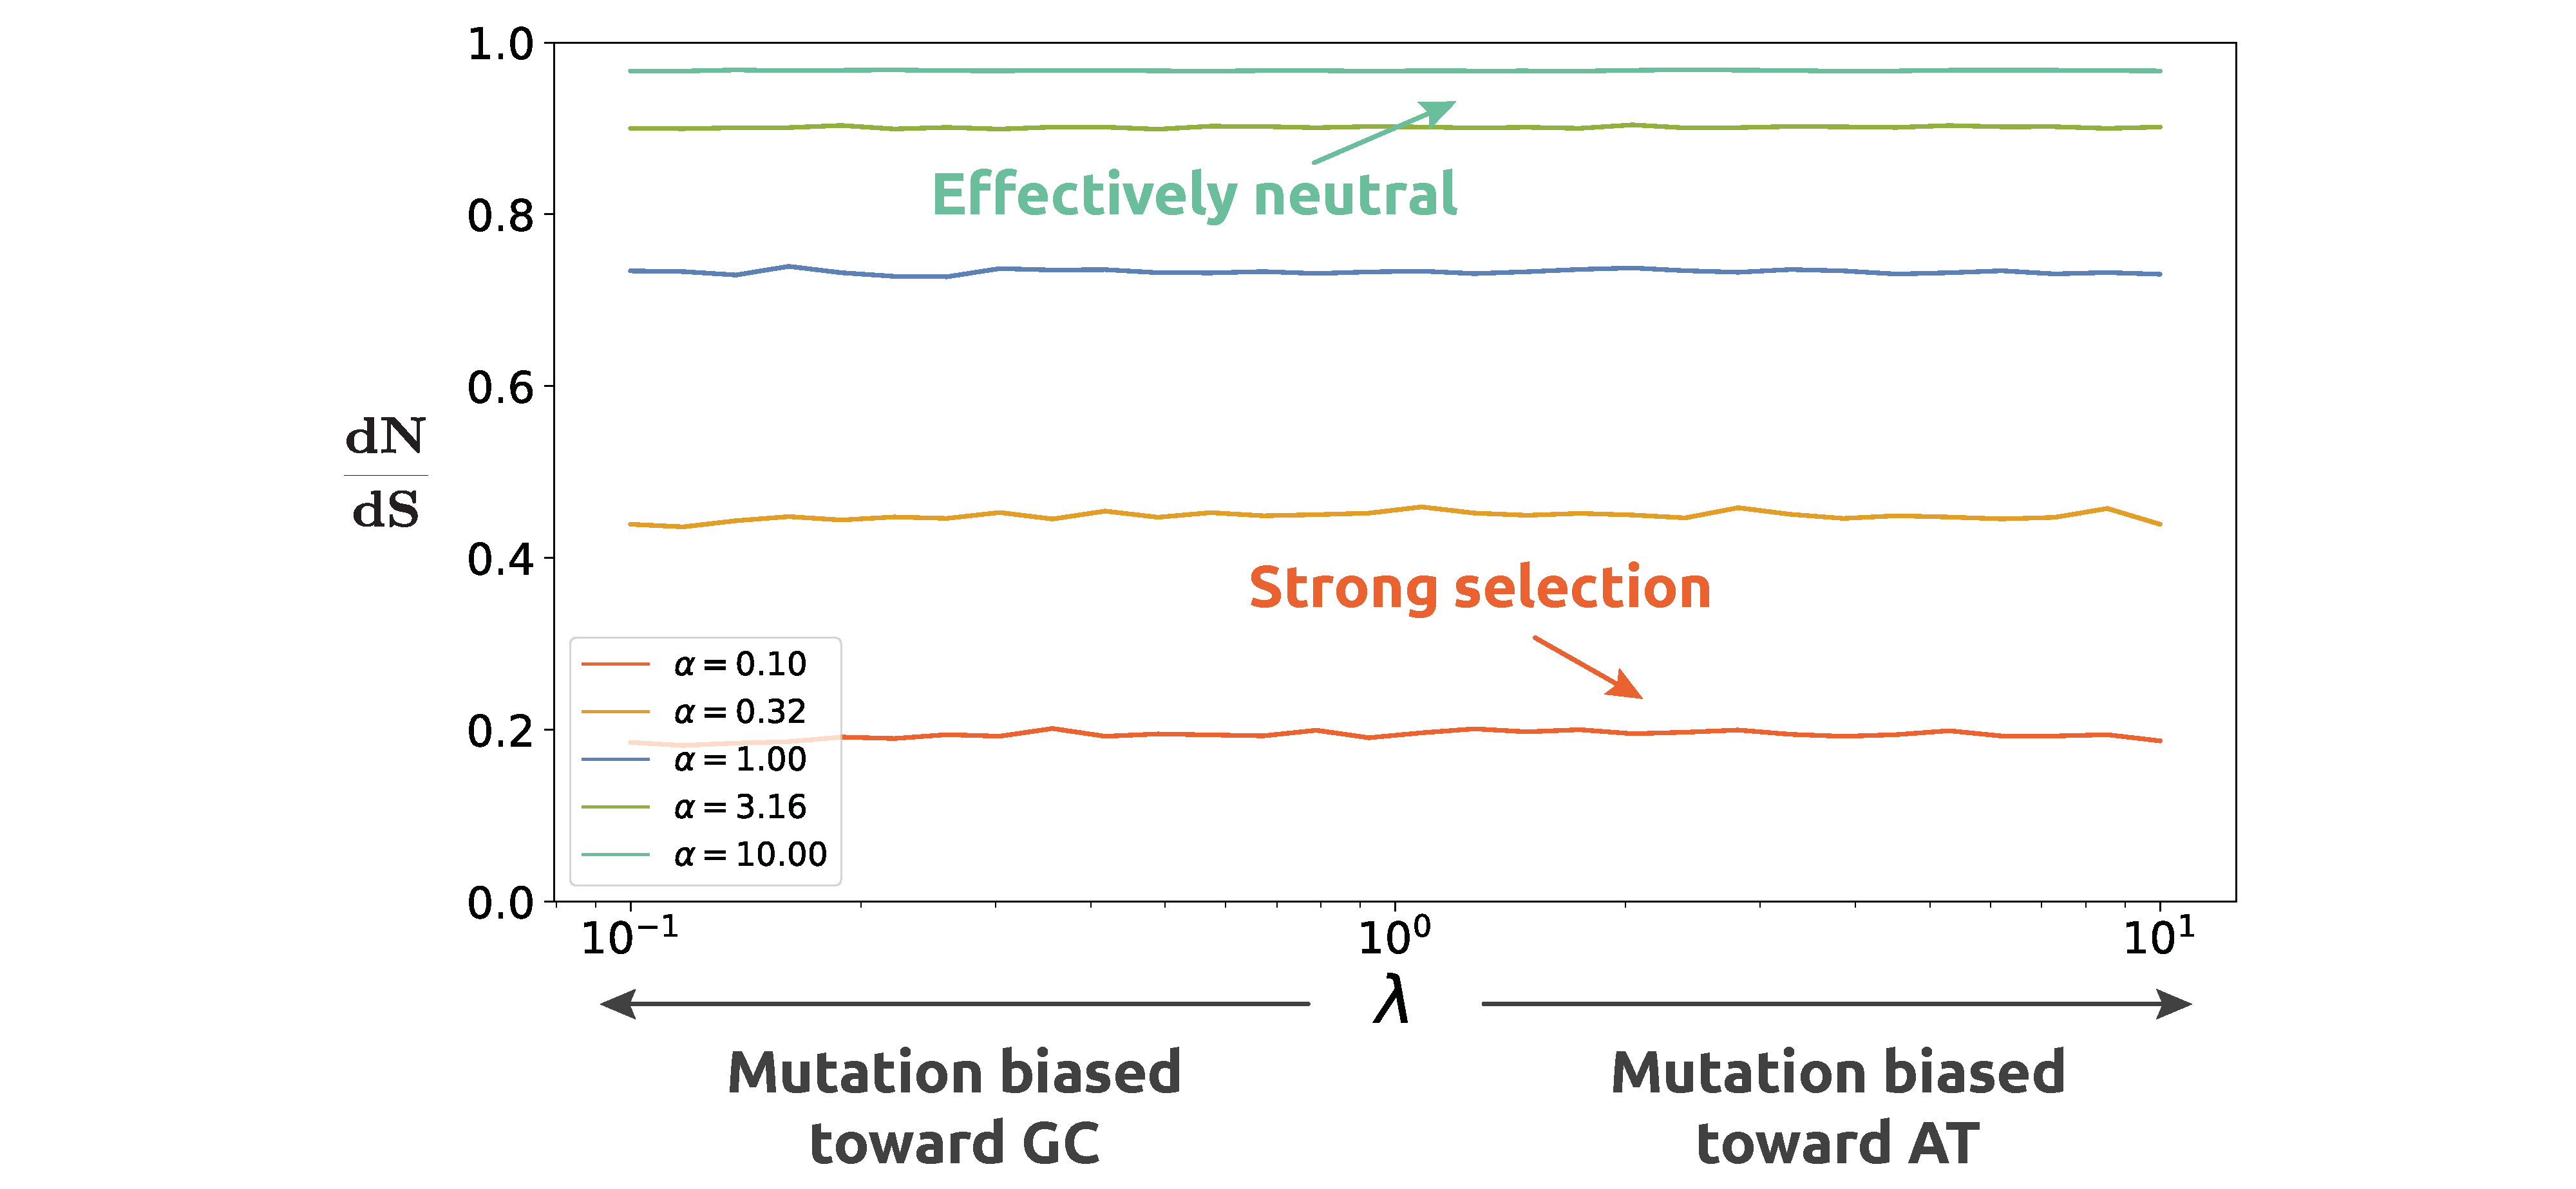
\includegraphics[width=\textwidth] {omega}
    \caption[$\omega$ as a function of the parameters]{
    $\omega$ as a function of the parameters.
    Non-synonymous fixation bias is always lower than 1.
    Non-synonymous fixation bias decrease with the strength of selection.
    Non-synonymous fixation bias is unaffected by mutational bias.
    }
    \label{fig-mut-bias:omega}
\end{figure}

$\bullet$ Fixation bias can be decomposed between fixation bias from weak nucleotides (A or T) to strong nucleotides (G or C).

$\bullet$ Fixation bias is opposed to mutational bias, such that mutation pushes toward less fit amino-acids that are disfavored (see figure \ref{fig-mut-bias:omega-WS-SW}).

\begin{figure}[H]
    \centering
    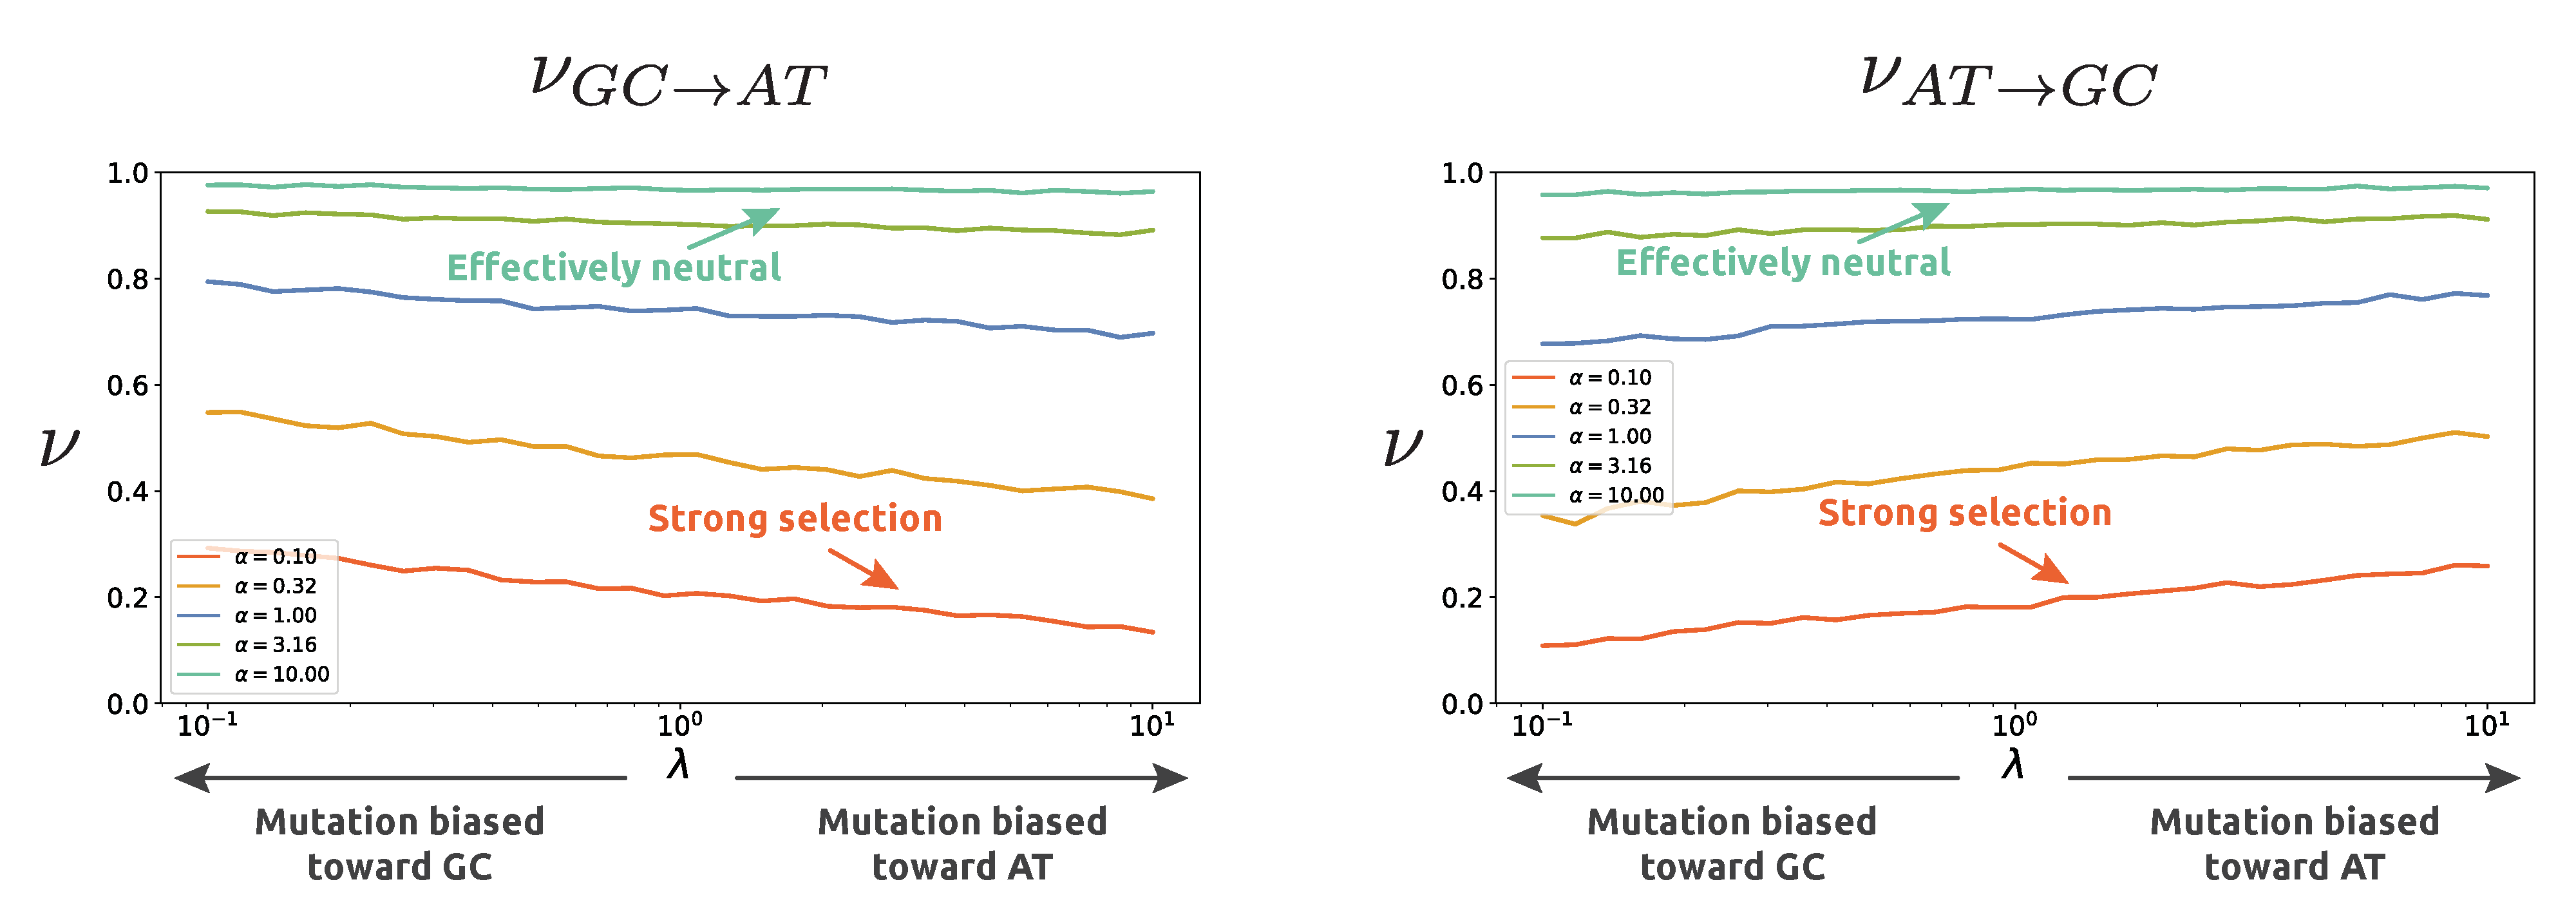
\includegraphics[width=\textwidth, page=1] {omega-WS-SW}
    \caption[Fixation bias of non-synonymous mutations]{
    Fixation bias of non-synonymous mutations.
    Mutation biased from GC to AT leads to a fixation bias in the opposite direction.
    More generally, mutation bias leads to balancing fixation bias.
    This is confounding factor with gBGC.}
    \label{fig-mut-bias:omega-WS-SW}
\end{figure}

\subsection{Parametric inference with phenomenological codon model}

$\bullet$ Known values of underlying $\lambda$ and simulated $\omega$ can be compared to estimates under different models, models knowing solely the protein coding DNA alignment (see figure \ref{fig-mut-bias:pipeline}).

\begin{figure}[H]
    \centering
    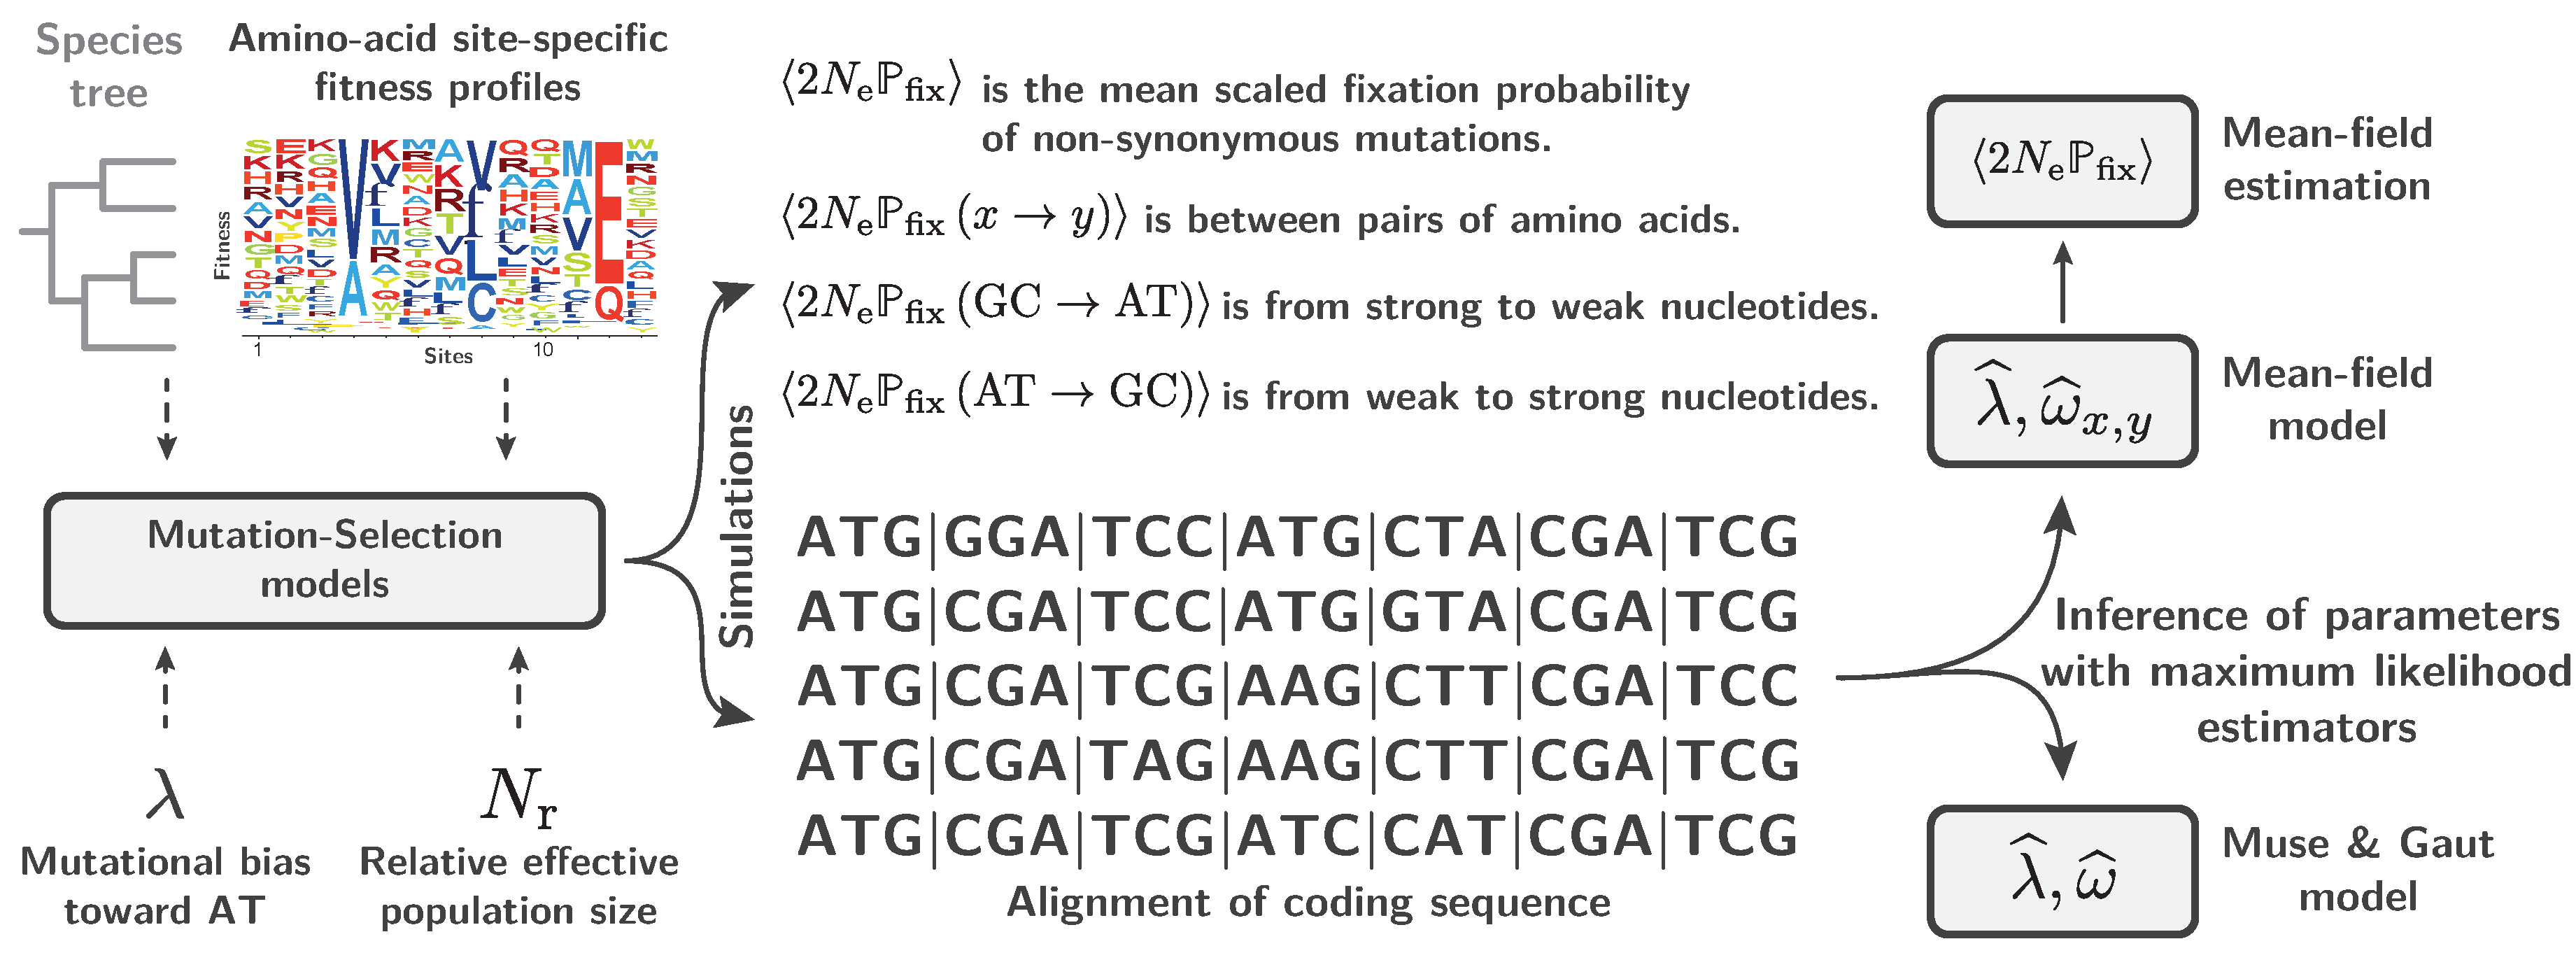
\includegraphics[width=\textwidth, page=1] {pipeline}
    \caption[Inferred value compared to known value]{
    Inferred value compared to known value.}
    \label{fig-mut-bias:pipeline}
\end{figure}

The $61$-by-$61$ \gls{codon} \gls{substitution} matrix of \citet{Muse1994} is defined entirely by the mutation matrix ($\Mutmatrix$), $\omega$ and the genetic code:
\begin{equation}
    \begin{dcases}
        \submatrix_{\itoj} & = 0 \text{ if $\ci$ and $\cj$ are not one mutation away} \\
        \submatrix_{\itoj} & = \mutmatrix_{\nucitoj} \text{ if $\ci$ and $\cj$ are syonymous} \\
        \submatrix_{\itoj} & = \omega \mutmatrix_{\nucitoj} \text{ if $\ci$ and $\cj$ are non-syonymous} \\
        \submatrix_{\ci, \ci} & = - \sum\limits_{\cj \neq \ci} \submatrix_{\itoj}
    \end{dcases}
    \label{eq:codon-muse-gaut}
\end{equation}

$\bullet$ Phenomenological codon models are not designed to tease out mutational bias, fixation bias is not implemented.

$\bullet$ From the maximum \gls{likelihood} estimates of the $4 \times 4$ mutation matrix ($\widehat{\Mutmatrix}$), we can estimate of the mutational bias toward $\mathrm{AT}$ $\left({\widehat{\lambda}_{\text{MG}}} \right)$.
Estimate of the mutational bias is halfway between observed bias of the alignment and true value (see figure \ref{fig-mut-bias:inference}, left panel).

$\bullet$ We can also estimate the fixation bias of non-synonymous mutations (${\widehat{\omega}_{\text{MG}}}$).
Error of the estimated non-synonymous fixation bias is 1.8\%.

\subsection{Parametric inference with mean-field codon model}

$\bullet$ Mean-field models are parameterized to account for fixation bias in different directions.

Under projected mutation-selection model, the $61$-by-$61$ \gls{codon} \gls{substitution} matrix of mechanistic \gls{codon} models is defined entirely by the mutation matrix ($\Mutmatrix$), the fixation bias between all pairs of amino-acids $\omega_{\aai, \aaj}$ and the genetic code:
\begin{equation}
    \begin{dcases}
        \submatrix_{\itoj} & = 0 \text{ if $\ci$ and $\cj$ are non neighbors}, \\
        \submatrix_{\itoj} & = \mu_{\itoj} \text{ if $\ci$ and $\cj$ are syonymous}, \\
        \submatrix_{\itoj} & = \mu_{\itoj} \omega_{\aai, \aaj} \text{ if $\ci$ and $\cj$ are non-syonymous}, \\
        \submatrix_{\ci, \ci} & = - \sum\limits_{\cj \neq \ci} \submatrix_{\itoj}.
    \end{dcases}
    \label{eq:codon-mean-field}
\end{equation}
Because of the structure of the genetic code, the total number of pairs of amino-acid that are one nucleotide away (neighbors) is not $190$ but $75$, because some amino-acids are not directly accessible trough a single non-synonymous mutation.
As a result, the number of parameters necessary to determines all fixation bias ($\omega_{\aai, \aaj}$) in both direction is $150$.
However, under the assumption of a reversible process, the number of parameters can be reduced to $75$ parameters of exchangeabilities ($\beta_{\aai, \aaj}$) and $20$ parameters of stationary distribution ($\epsilon_{\aai}$).
\begin{align}
    \omega_{\aai, \aaj} = \epsilon_{\aaj} \beta_{\aai, \aaj}, \\
    \text{ where } \beta_{\aai, \aaj} = \beta_{\aaj, \aai}.
\end{align}
The process is reversible:
\begin{align}
    \epsilon_{\aai} \omega_{\aai, \aaj} & = \epsilon_{\aai} \epsilon_{\aaj} \beta_{\aai, \aaj}, \\
     & = \epsilon_{\aaj} \omega_{\aaj, \aai}
\end{align}

$\bullet$ From the maximum \gls{likelihood} estimates of the mutation matrix ($\widehat{\Mutmatrix}$), we can estimate the mutational bias $\left({\widehat{\lambda}_{\text{MF}}} \right)$.
Estimate of the mutational bias can tease out observed bias of the alignment and true value (see figure \ref{fig-mut-bias:inference}, left panel).

$\bullet$ We can also estimate the fixation bias of non-synonymous mutations $\left({\widehat{\omega}_{\text{MF}}} \right)$ (see section \ref{sec-mut-bias:mean-field-omega}) which is a compound parameter of the mutation matrix and the fixation bias in the different direction.
Error of the estimated non-synonymous fixation bias is 3.0\%.
Also, in empirical data we observed that the fixation bias between weak and strong nucleotide is not equal, and is opposite of the nucleotide bias (see table \ref{table-mut-bias:estimation}).
\begin{figure}[H]
    \centering
    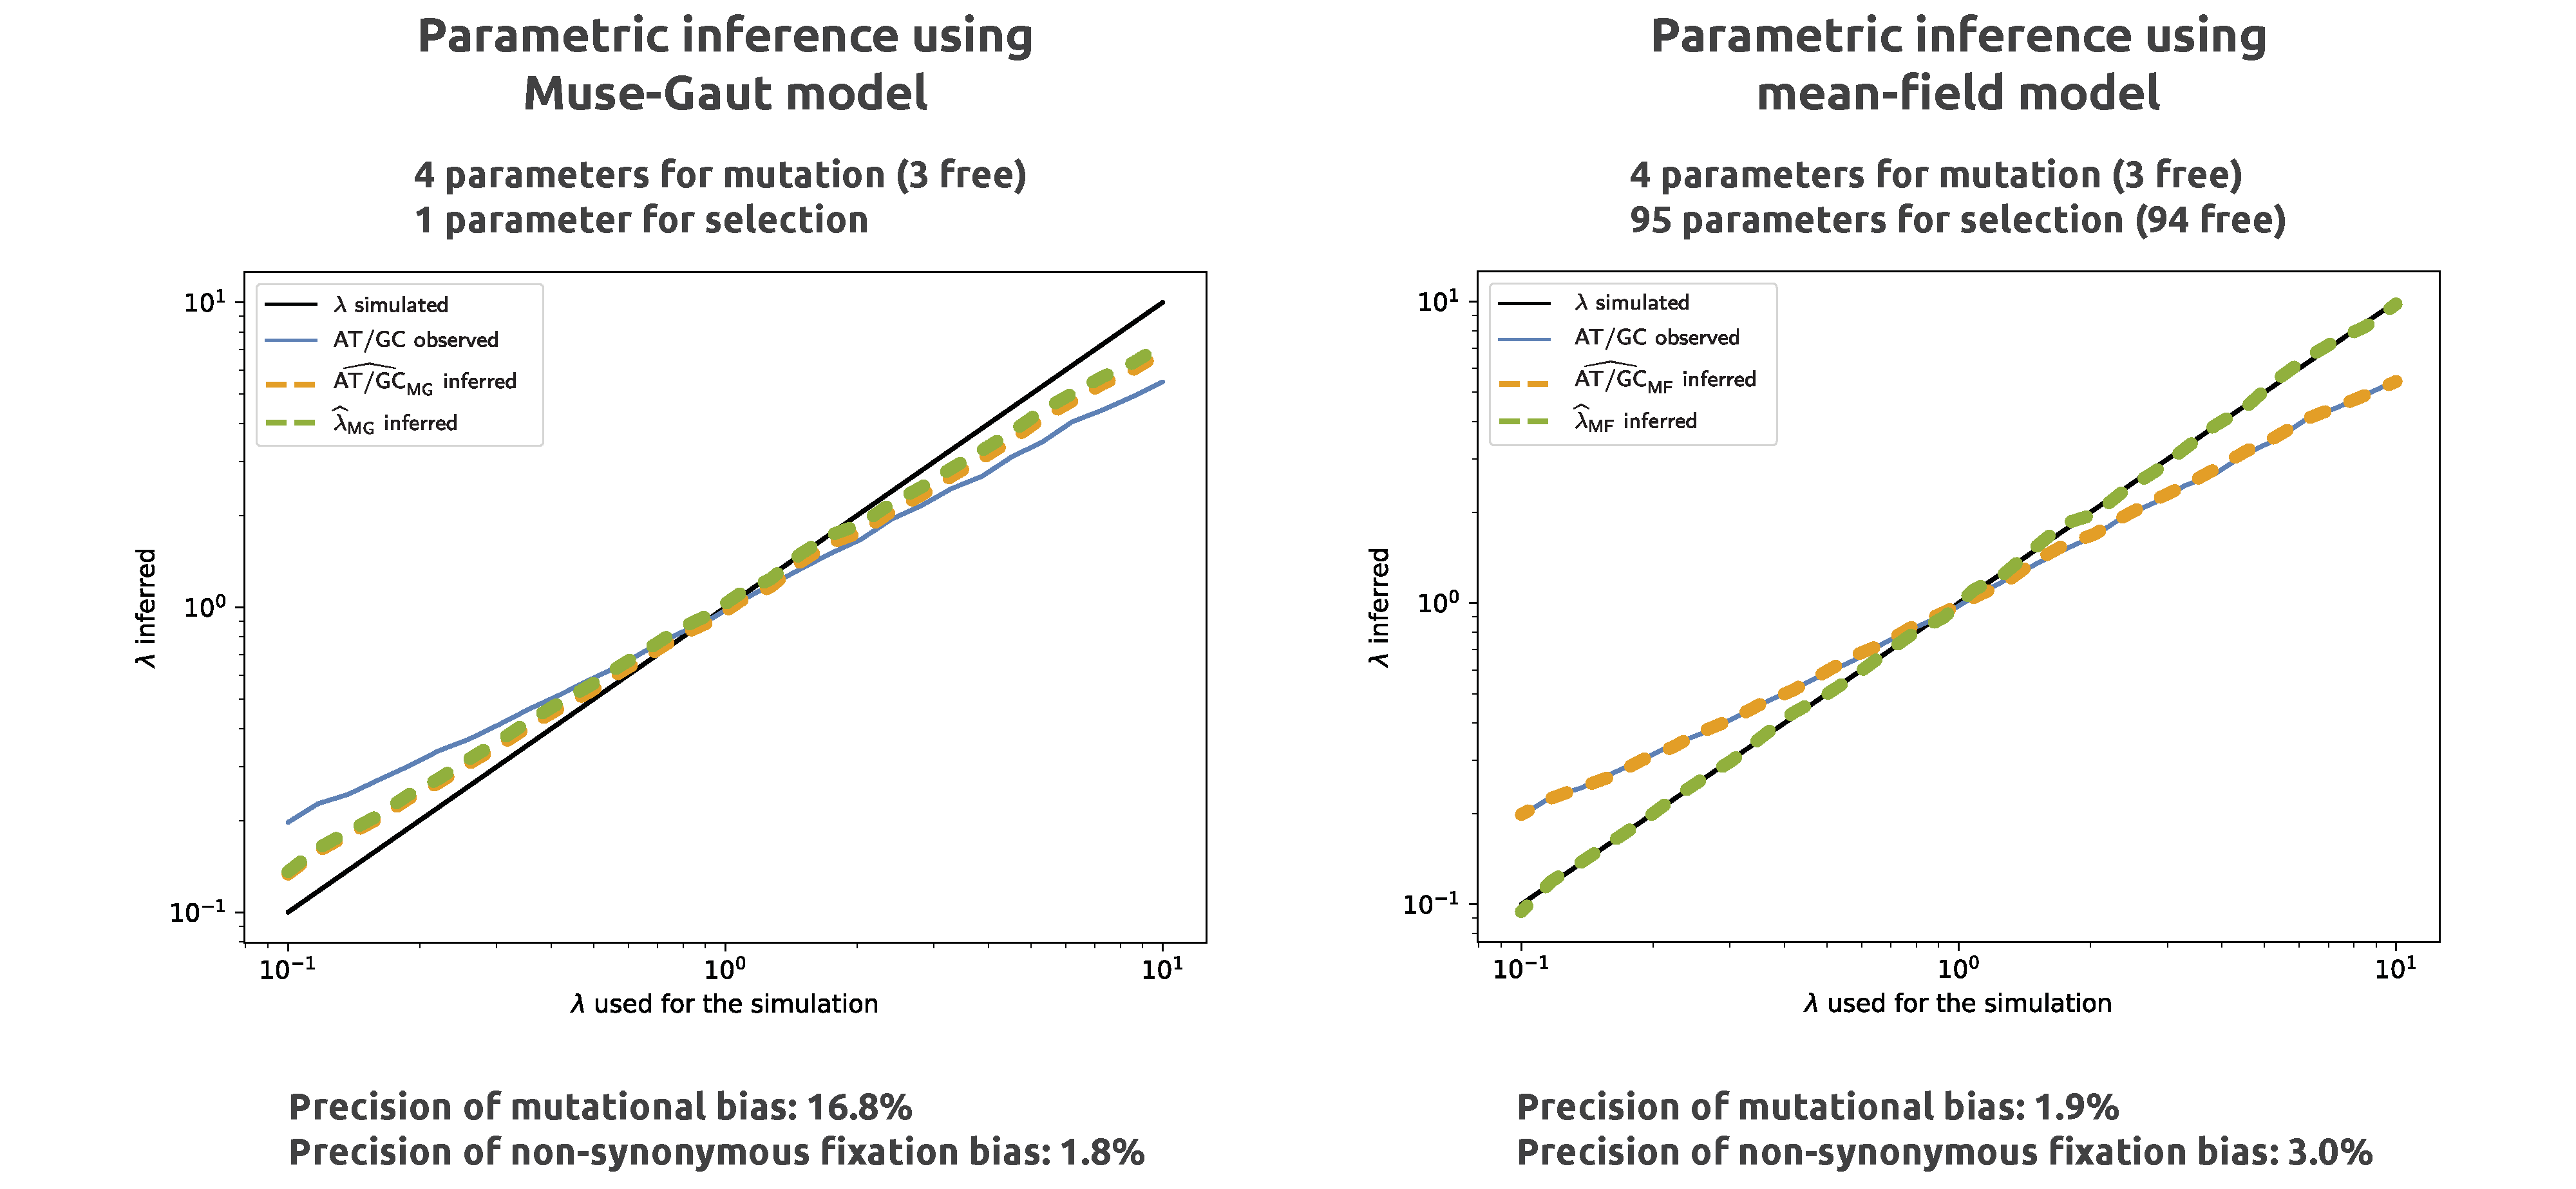
\includegraphics[width=\textwidth] {Simulation-vs-Inference}
    \caption[Estimation of mutation and fixation bias]{
    Estimation of mutational bias.
    Modeling a single fixation bias leads to skewed estimation of mutation bias.
    Modeling multiple fixation bias leads to precise estimation of mutation bias}
    \label{fig-mut-bias:inference}
\end{figure}

\begin{table}[H]
    \centering
    \noindent\adjustbox{max width=\textwidth}{%
    \begin{tabu}{|c||c|c|}
        \hline
        \textbf{Estimated parameter} & Nucleoprotein & Lactamase \\
        \hline \textbf{AT/GC of the alignment} & 1.15 & 0.79 \\
        \hline \textbf{Muse-Gaut mutational bias $\left({\widehat{\lambda}_{\text{MG}}} \right)$ } & 1.39 & 0.85 \\
        \hline \textbf{Mean-field mutational bias $\left({\widehat{\lambda}_{\text{MF}}} \right)$} & 1.64 & 0.68 \\
        \hline \textbf{Mean-field fixation bias from AT to GC $\left(\widehat{\omega}_{\textbf{AT} \rightarrow \textbf{GC}}\right)$} & 0.14 & 0.31 \\
        \hline \textbf{Mean-field fixation bias from GC to AT $\left(\widehat{\omega}_{\textbf{GC} \rightarrow \textbf{AT}}\right)$} & 0.10 & 0.44 \\
        \hline
    \end{tabu}}
    \caption[Estimated parameters]{
    Nucleoprotein alignment of 498 amino-acids available for 180 species (left column).
    Lactamase alignment of 263 amino-acids available for 85 species (right column).
    }
    \label{table-mut-bias:estimation}
\end{table}

Maximum likelihood estimation has been performed with the software Hyphy \citep{Pond2005}.
The python scripts generating the Hyphy batch files (for both Muse \& Gaut and mean-field), as well as scripts to analyse experiments are available at \url{https://github.com/ThibaultLatrille/NucleotideBias}

\section{Conclusion}

$\bullet$ The observed composition of the alignment is the result of the articulation between mutation and selection.

$\bullet$ Mutational bias is balanced by a fixation bias (selection) in the opposite direction, potentially a confounding effect with gBGC.

$\bullet$ Inference of mutational bias requires to model fixation bias in different direction.

$\bullet$ Our mean-field parametric framework is not site-wise, but can be used to untangle mutation and selection, potentially in the presence of fluctuating selection or epistasis.

\section{Materials \& Methods}

\subsection{Modeling mutational bias}
\label{sec-mut-bias:mut-matrix}
The mutation rate between nucleotides is always proportional to $\mu$.
Moreover, mutations from any nucleotide to another weak nucleotide is increased by the factor $\lambda$ compared with mutations to another strong nucleotides.
The rate at which a nucleotide doesn't change is given such the sum of all rates is zero.
The mutation rate matrix is:
\begin{equation}
    \label{nucMatrix}
    \Mutmatrix =
    \begin{pmatrix}
    {-\mu(2 + \lambda)}
        & {\mu} & {\mu} & {\mu \lambda} \\
        {\mu \lambda} & {-\mu(1 + 2\lambda)} & {\mu} & {\mu \lambda} \\
        {\mu \lambda} & {\mu} & {-\mu(1 + 2\lambda)} & {\mu \lambda} \\
        {\mu \lambda} & {\mu} & {\mu} & {-\mu(2 + \lambda)}
    \end{pmatrix}.
\end{equation}
The stationary distribution $ \Subequi$ must be annihilated by the mutation matrix $\Mutmatrix$, which gives the stationary distribution:
\begin{align}
    \Mutequi \Mutmatrix & = 0, \\
    \iff \Mutequi & = \left( \dfrac{\lambda}{2+2\lambda}, \dfrac{1}{2+2\lambda}, \dfrac{1}{2+2\lambda}, \dfrac{\lambda}{2+2\lambda} \right).
    \label{nucStationarity}
\end{align}
The process is reversible and fulfills detailed balance conditions for any pair of different nucleotides:
\begin{align}
    \mutequi_a \mutmatrix_{a, b} =\mutequi_b \mutmatrix_{b, a}.
    \label{nucMutBalance}
\end{align}
It is important to note that ratio of weak over strong nucleotides frequency at stationarity is equal to $\lambda$:
\begin{align}
    \label{lambda}
    \dfrac{ \mutequi_A + \mutequi_T }{ \mutequi_C + \mutequi_G }
    & = \dfrac{ \lambda ( 2 + 2 \lambda)^{-1} + \lambda ( 2 + 2 \lambda)^{-1}}{ ( 2 + 2 \lambda)^{-1} +  ( 2 + 2 \lambda)^{-1}}, \ \textrm{from eq.}\ \ref{nucStationarity},\\
    & = \lambda.
\end{align}

\subsection{Modeling selection at the amino-acid level}
\label{sec-mut-bias:aa-selection}
The mutation rate between a pair of \glspl{codon} is given by the underlying mutation rates between nucleotides.
However the rate mutation rate is null if the pair of \glspl{codon} differs by more than one nucleotide:
To note, the \gls{substitution} rate between \glspl{codon} would be equal to the mutation rate if \glspl{codon} are selectively \gls{neutral}.
However, we subsequently take into the selection acting on \gls{codon} by modeling it at the amino-acid level, where each amino-acid $\aai$ encoded by codon $\ci $are given a fitness ($\Fiti$).
By modeling fitness at the amino-acid level, we assume that all \glspl{codon} encoding for one particular amino-acid are selectively \gls{neutral}.
In this modeling framework, the genetic code is of particular importance since the number of \glspl{codon} encoding for a particular amino-acid varies greatly.
As an example, Tryptophan is encoded by one \gls{codon}, while Leucine is encoded by 6 \glspl{codon}.
Intuitively, this variation makes the mutation bias more effective in \glspl{codon} encoding for many amino-acids since there are many mutations possible that are selectively \gls{neutral} (same amino-acid).
While the other hand, the mutation bias is more constrained if the amino-acid is encoded by a few \glspl{codon} since there is only a few mutations possible that are selectively \gls{neutral}.\\

To take into account the heterogeneity of selection between different sites of the protein, we assume that each site $\site$ of the sequence is evolving under a different fitness landscape ($\Fiti\siteexp$).
At one particular site, under a static fitness landscape, the \gls{substitution} rate between \glspl{codon} are given by the product of the mutation rate and the probability of fixation:
\begin{equation}
    \begin{dcases}
        \submatrix_{\itoj} & = 0 \text{ if $\ci$ and $\cj$ are non neighbors} \\
        \submatrix_{\itoj} & = \mu_{\itoj} \text{ if $\ci$ and $\cj$ are syonymous} \\
        \submatrix_{\itoj} & = \mu_{\itoj} \dfrac{\Fitj - \Fiti}{1 - \e^{\Fiti - \Fitj} } \text{ if $\ci$ and $\cj$ are non-syonymous} \\
        \submatrix_{\ci, \ci} & = - \sum\limits_{\cj \neq \ci} \submatrix_{\itoj}
    \end{dcases}
    \label{codonSubRates}
\end{equation}
At the root the tree, the sequence is obtained by sampling from the equilibrium stationnary distribution
The stationary distribution $\Subequi$ must be annihilated by the mutation matrix $\Submatrix$, which gives the stationary distribution at site $\site$:
\begin{align}
    \Subequi\siteexp \bm{Q}\siteexp
    & = 0 ,\\
    \iff \subequi_{\ci}\siteexp
    & = \mathcal{Z}\siteexp \lambda^{\nbrWeak_{\ci}} \e^{\Fiti\siteexp},\\
    & \mathrm{ where } \ \mathcal{Z}\siteexp = \left( \sum\limits_{\cj=1}^{61} \lambda^{\nbrWeak_{\cj}} \e^{\Fitj\siteexp} \right)^{-1},
    \label{codonStationarity}
\end{align}
where $\nbrWeak_{\ci}$ is the number of weak nucleotide (A or T) in the codon (between 0 and 3).

Moreover, the \gls{substitution} process is reversible and fulfills detailed balance conditions at each site $\site$:
\begin{align}
    \subequi_{\ci}\siteexp \submatrix_{\itoj}\siteexp = \subequi_{\cj}\siteexp \submatrix_{\cj, \ci}\siteexp
    \label{codonSubBalance}
\end{align}

\subsection{Simulation}
\label{sec-mut-bias:simu}
We seek to simulate the evolution of protein-coding sequences along a specie tree.
Starting with one sequence at the root of the tree, the sequences evolves independently along the different branches of the tree by point substitutions, until they reach the leaves.
At the end of the simulation, we get one sequence for each leaf of the tree, meaning one sequence per specie.
Such evolutionary process is an idealized version of the reality, in the sens that the whole heterogeneity of sequences in the population is wiped away, with only one sequence representing the whole population.
For a protein-coding \acrshort{DNA} sequence, a \gls{substitution} is modeled as the product of mutation at the nucleotide level, and selection of the amino-acid level.
On one hand, the mutation rate between nucleotides as assumed to be same for all sites of the sequences.
On the other hand, the selection for amino-acids is assumed to be varying along the sequences.
During the simulation, from a given sequence the substitution rate toward all possible mutant (one nucleotide change) is computed and the next substitution is chosen by Gillespie algorithm.

\subsection{Fixation bias under the mean-field model}
\label{sec-mut-bias:mean-field-omega}

The fixation bias is:
\begin{align}
    \omega_{\text{MF}} & = \dfrac{ \sum\limits_{i} \sigma_{\ci[1]}\sigma_{\ci[2]}\sigma_{\ci[3]} \epsilon_{\aaj} \sum\limits_{j \in \NonSyn_{\ci}} \mu_{\itoj} \epsilon_{\aaj} \beta_{\aai, \aaj} }{\sum\limits_{i} \pi_{i} \sum\limits_{j \in \NonSyn_{\ci} } \mu_{\itoj}}
\end{align}

The fixation bias from weak to strong is $\omega_{\textbf{AT} \rightarrow \textbf{GC}}$ is obtained similarly by restricting the sum to one nucleotide mutation only from weak to strong.
Conversely, the fixation bias from strong to weak is obtained by restricting one nucleotide mutation only from weak to strong.